% Faz com que o ínicio do capítulo sempre seja uma página ímpar
\cleardoublepage
% Inclui o cabeçalho definido no meta.tex
\pagestyle{fancy}
% Números das páginas em arábicos
\pagenumbering{arabic}

\chapter{Introdução}\label{intro}
É notável o crescente avanço do poder computacional dos computadores nos últimos anos. Já é comum inclusive computadores pessoais terem mais de um processador. Desenvolver programas ou algoritmos que não utilizam completamente os recursos disponíveis nas máquinas resulta em um desperdício de capacidade de processamento da máquina.

O maior desafio atual é desenvolver técnicas que possuam boa escalabilidade, ou seja, ter um aumento no desempenho quando mais recursos computacionis forem disponíveis, mantendo os resultados obtidos pelo algoritmo sequencial.

Esse trabalho está focado em malhas bidimensionais, mais precisamente triangulações. Essas malhas são bastante utilizadas em diversas áreas e aplicações. Na engenharia são bastante utilizadas em métodos de elementos finitos (MEF). Em computação gráfica são muito utilizadas para a visualização e modelagem objetos e ambientes. Há usos também em  sistemas de informações geográficas e projetos assistidos por computadores para a modelagem de objetos industriais.

A qualidade da malha gerada é bastante importante. Em um MEF, por exemplo, se uma malha tiver uma grande quantidade de elementos ruins (polígonos, em malhas bidimensionais), é possível que este não convirja. Por necessitar de malhas bastante refinadas, é comum que MEFs usem malhas grandes, com milhões de elementos.

Em geração de malha para aplicações científicas, é preciso ter uma boa técnica para garantir que os elementos gerados sejam de boa qualidade, ou seja, no caso bidimensional, que os triângulos sejam bons. Pode-se dizer que um triângulo é bom quando ele é quase equilátero, caso contrário, ele pode ser ruim (Figura~\ref{fig:imagem10}).

 \begin{figure}[htbp]
     \centering
     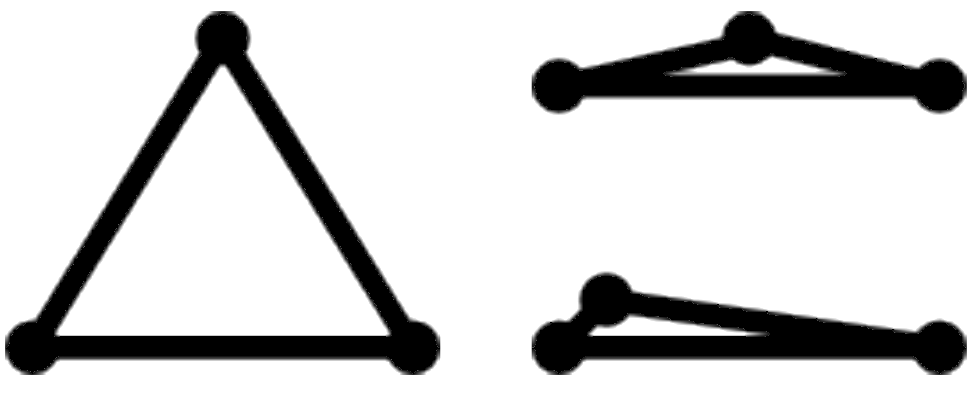
\includegraphics[width=0.7\textwidth]{imagem10}
     \caption{Triângulo bom e triângulos ruins} 
     \label{fig:imagem10}
 \end{figure}

O restante deste trabalho está dividido em quatro seções. O capítulo seguinte faz uma apresentação do que se tem feito atualmente na área de decomposição de domínios. O Capítulo 3 descreve os algoritmos existentes para geração de malhas bidimensionais, mais precisamente, triangulações. Finalmente, no Capítulo 4 é feito uma conclusão e é defino a linha de estudo, também é apresentado o cronograma de trabalho.

